\datos{color}{}{}
\subsection{\textit{MIT Cheetah}}
\textit{MIT Cheetah}, desarrollado por el \textit{Biomimetic Robotics Lab} del 
\textit{Massachusetts Institute of Technology} (\textit{MIT}), 
Figura \ref{cheetah}, es uno de los robots cuadrúpedos más influyentes en la investigación moderna 
sobre locomoción dinámica. Su primera versión funcional se presentó en 2012, y desde entonces ha 
evolucionado a \textit{Cheetah 2}, \textit{Cheetah 3} y \textit{Mini Cheetah}, convirtiéndose 
en una plataforma de referencia para el estudio del control híbrido, la planificación dinámica 
y la locomoción de alta velocidad. El robot integra actuadores eléctricos de alta potencia, 
sensores de torque, cámaras y sensores inerciales, junto con un ordenador central encargado de 
la percepción y la planificación. \\

Sus usos principales incluyen la investigación en control predictivo, locomoción dinámica, 
planificación de movimientos, aprendizaje por refuerzo y exploración autónoma. Gracias a su 
capacidad para correr, saltar, recuperar el equilibrio tras perturbaciones y desplazarse por 
terrenos irregulares, \textit{MIT Cheetah} ha sido ampliamente utilizado en experimentos de 
laboratorio y en estudios sobre estabilidad dinámica y control avanzado de cuadrúpedos. \\

A diferencia de los robots centralizados y distribuidos presentados anteriormente, 
\textit{MIT Cheetah} implementa una arquitectura de 
control híbrida. El ordenador central ejecuta los módulos de percepción, integración multisensorial,
planificación de trayectorias y control predictivo basado en modelos, siguiendo la descomposición 
vertical clásica. Sin embargo, cada articulación dispone de controladores locales que procesan 
directamente la información sensorial y generan respuestas rápidas para mantener la estabilidad, 
absorber impactos o corregir perturbaciones. Los niveles superiores planifican el movimiento global
mediante técnicas 
como el \textit{Model Predictive Control} (\textit{MPC}), mientras que los niveles inferiores garantizan la 
ejecución reactiva y segura del patrón de marcha. Esta combinación de planificación deliberativa 
y control reactivo, es decir, arquitectura híbrida, permite al robot adaptarse rápidamente a 
cambios del entorno. \\

\begin{wrapfigure}{r}{0.3\textwidth}
\centering
\vspace{-10pt}
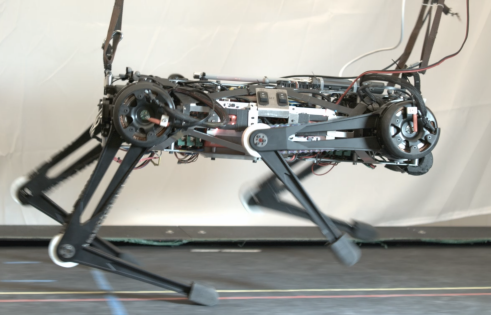
\includegraphics[width=0.3\textwidth]{Images/cheetah.png}
\caption{\label{cheetah}\textit{MIT Cheetah 3}.}
\vspace{-10pt}
\end{wrapfigure}

\textit{MIT Cheetah} utiliza un sistema de locomoción cuadrúpedo con doce grados de libertad, 
accionados mediante actuadores eléctricos de alta eficiencia y sensores de torque. La combinación 
de control de impedancia, estimación del estado corporal y planificación dinámica permite al robot
caminar, correr, saltar, girar con precisión y mantener la estabilidad ante perturbaciones externas. 
Su locomoción reactiva y su capacidad para ejecutar maniobras dinámicas complejas lo convierten en 
un ejemplo representativo de las arquitecturas híbridas modernas aplicadas a robots cuadrúpedos de 
alto rendimiento.

\subsection*{Referencias}
\cite{Cheetah2018} \fullcite{Cheetah2018}.\\
\cite{Cheetah2015} \fullcite{Cheetah2015}.